\documentclass{beamer}

\mode<presentation>
{
  \usetheme{default}
  \usecolortheme{default}
  \usefonttheme{default}
  \setbeamertemplate{navigation symbols}{}
  \setbeamertemplate{caption}[numbered]
  \setbeamertemplate{footline}[page number]
  \setbeamercolor{frametitle}{fg=white}
  \setbeamercolor{footline}{fg=black}
} 

\usepackage[english]{babel}
\usepackage[utf8x]{inputenc}
\usepackage{tikz}
\usepackage{listings}
\usepackage{courier}
\usepackage{array}
\usepackage{bold-extra}
\usepackage{minted}
\usepackage{textcomp}

\xdefinecolor{darkblue}{rgb}{0.1,0.1,0.7}
\xdefinecolor{darkgreen}{rgb}{0,0.5,0}
\xdefinecolor{darkgrey}{rgb}{0.35,0.35,0.35}
\xdefinecolor{darkorange}{rgb}{0.8,0.5,0}
\xdefinecolor{darkred}{rgb}{0.7,0,0}
\xdefinecolor{dianablue}{rgb}{0.18,0.24,0.31}
\definecolor{commentgreen}{rgb}{0,0.6,0}
\definecolor{stringmauve}{rgb}{0.58,0,0.82}

\lstset{ %
  backgroundcolor=\color{white},      % choose the background color
  basicstyle=\ttfamily\small,         % size of fonts used for the code
  breaklines=true,                    % automatic line breaking only at whitespace
  captionpos=b,                       % sets the caption-position to bottom
  commentstyle=\color{commentgreen},  % comment style
  escapeinside={\%*}{*)},             % if you want to add LaTeX within your code
  keywordstyle=\color{blue},          % keyword style
  stringstyle=\color{stringmauve},    % string literal style
  showstringspaces=false,
  showlines=true
}

\lstdefinelanguage{scala}{
  morekeywords={abstract,case,catch,class,def,%
    do,else,extends,false,final,finally,%
    for,if,implicit,import,match,mixin,%
    new,null,object,override,package,%
    private,protected,requires,return,sealed,%
    super,this,throw,trait,true,try,%
    type,val,var,while,with,yield},
  otherkeywords={=>,<-,<\%,<:,>:,\#,@},
  sensitive=true,
  morecomment=[l]{//},
  morecomment=[n]{/*}{*/},
  morestring=[b]",
  morestring=[b]',
  morestring=[b]"""
}

\title[2017-05-03-future-trends]{Lowering boundaries between \\ data analysis ecosystems}
\author{Jim Pivarski}
\institute{Princeton University -- DIANA Project}
\date{May 3, 2017}

\begin{document}

\logo{\pgfputat{\pgfxy(0.11, 8)}{\pgfbox[right,base]{\tikz{\filldraw[fill=dianablue, draw=none] (0 cm, 0 cm) rectangle (50 cm, 1 cm);}}}\pgfputat{\pgfxy(0.11, -0.6)}{\pgfbox[right,base]{\tikz{\filldraw[fill=dianablue, draw=none] (0 cm, 0 cm) rectangle (50 cm, 1 cm);}
\includegraphics[height=0.99 cm]{diana-hep-logo.png}\tikz{\filldraw[fill=dianablue, draw=none] (0 cm, 0 cm) rectangle (4.9 cm, 1 cm);}}}}

\begin{frame}
  \titlepage
\end{frame}

\logo{\pgfputat{\pgfxy(0.11, 8)}{\pgfbox[right,base]{\tikz{\filldraw[fill=dianablue, draw=none] (0 cm, 0 cm) rectangle (50 cm, 1 cm);}
\includegraphics[height=1 cm]{diana-hep-logo.png}}}}

% Uncomment these lines for an automatically generated outline.
%\begin{frame}{Outline}
%  \tableofcontents
%\end{frame}

%%%%%%%%%%%%%%%%%%%%%%%%%%%%%%%%%%%%%%%%%%%%%%%%%%%%%%%

%% \begin{frame}{Data analysis ecosystems}
%% 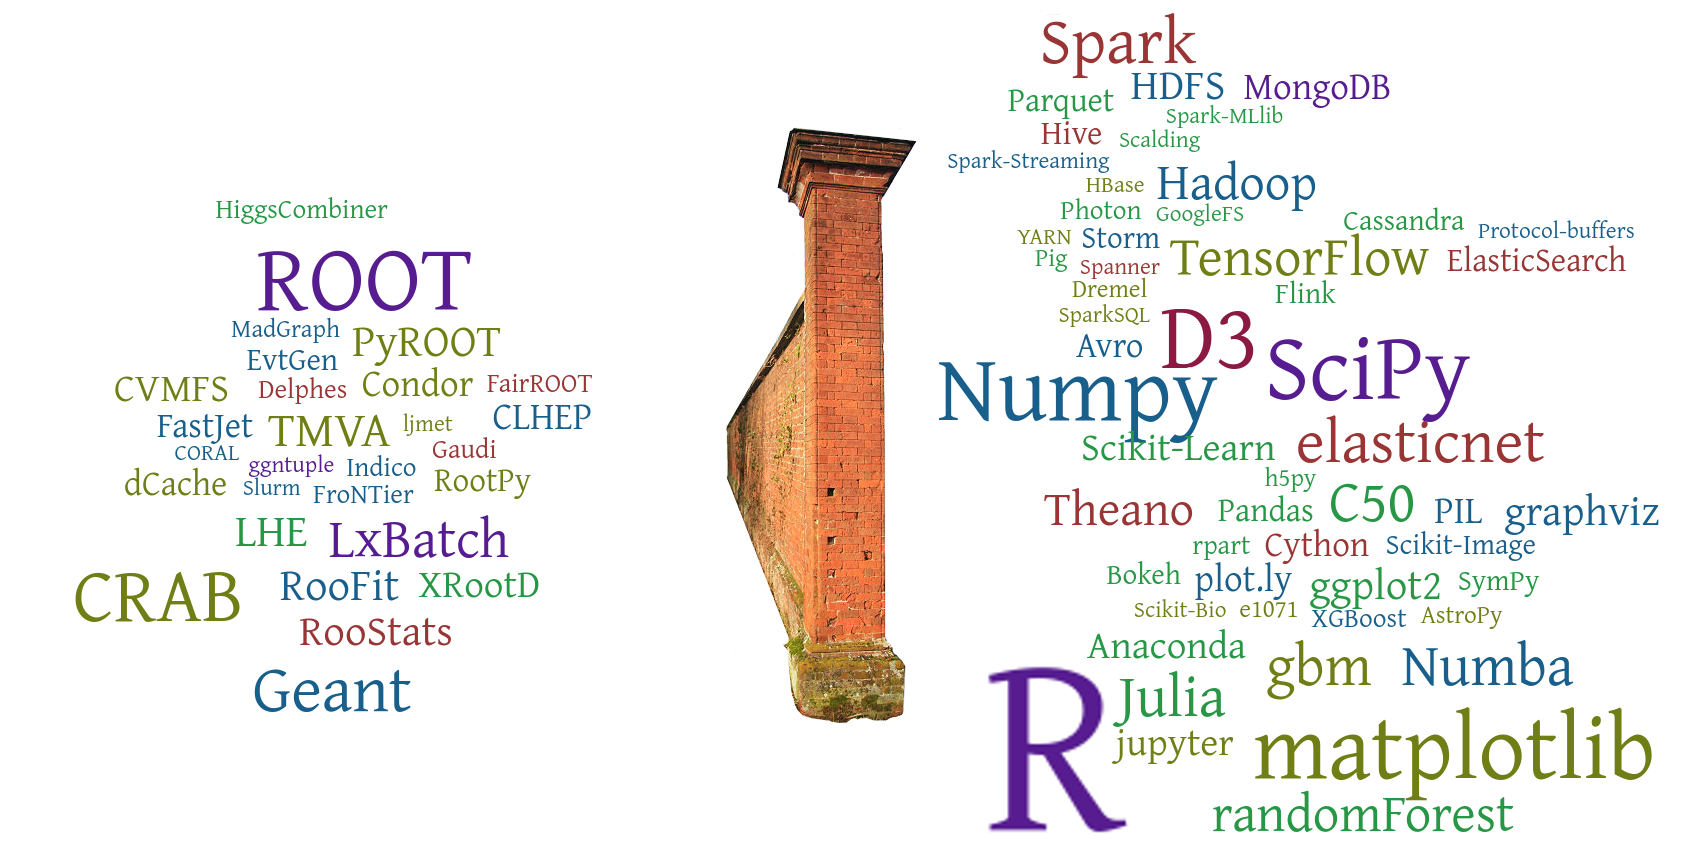
\includegraphics[width=\linewidth]{separation.png}
%% \end{frame}

%% \begin{frame}{}
%% \begin{center}
%% \large \textcolor{darkblue}{Physicists developed their own software for a good reason:}

%% \textcolor{darkblue}{no one else was tackling such large problems.}
%% \end{center}
%% \end{frame}

%% \begin{frame}{Not so today\ldots}
%% \vspace{0.5 cm}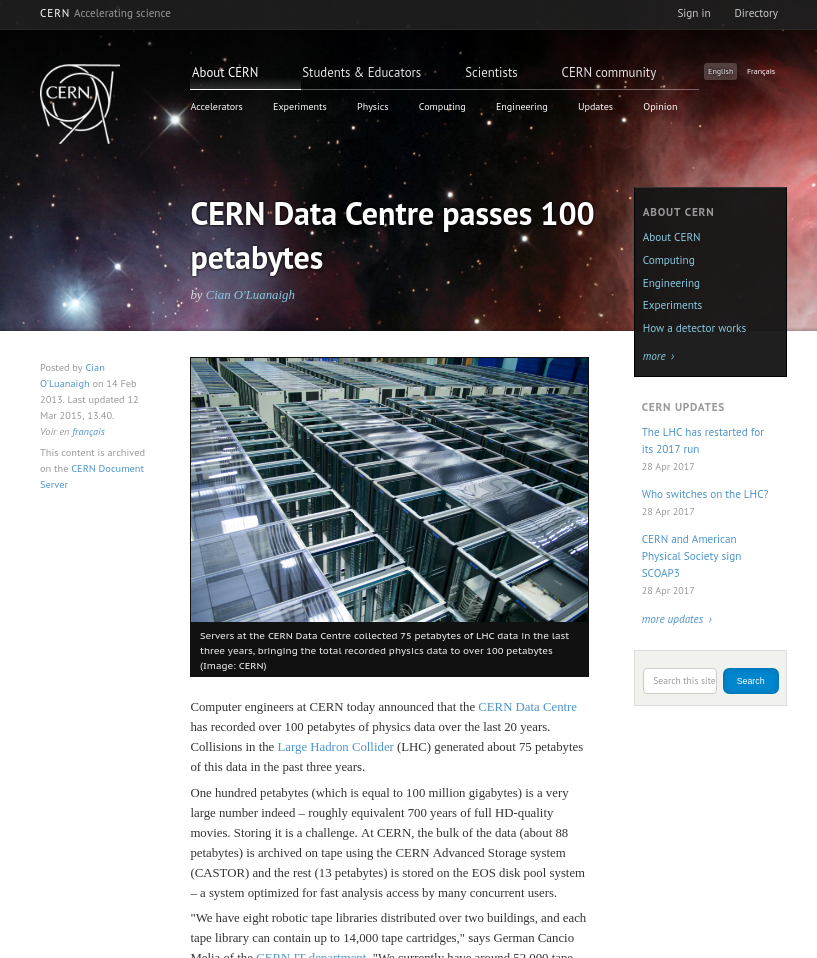
\includegraphics[width=0.75\linewidth]{cern_petabytes.png}

%% \vspace{-6.4 cm}\only<2>{\hfill 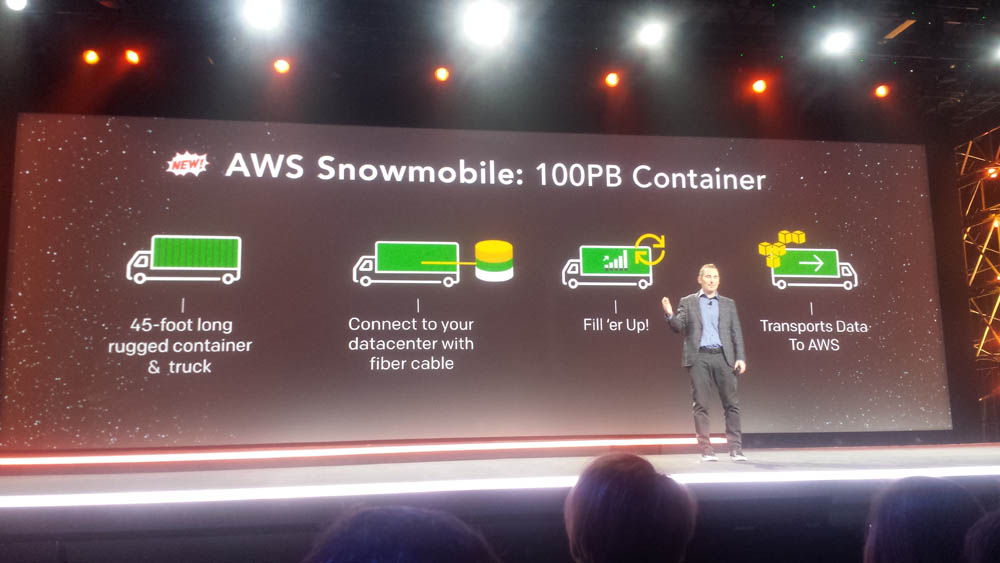
\includegraphics[width=0.75\linewidth]{aws-snowmobile.jpg}}\vspace{6.4 cm}
%% \end{frame}

%% \begin{frame}{Case in point: ROOT and Spark}
%% \vfill
%% \textcolor{darkblue}{Relative rate of web searches (Google Trends):}

%% 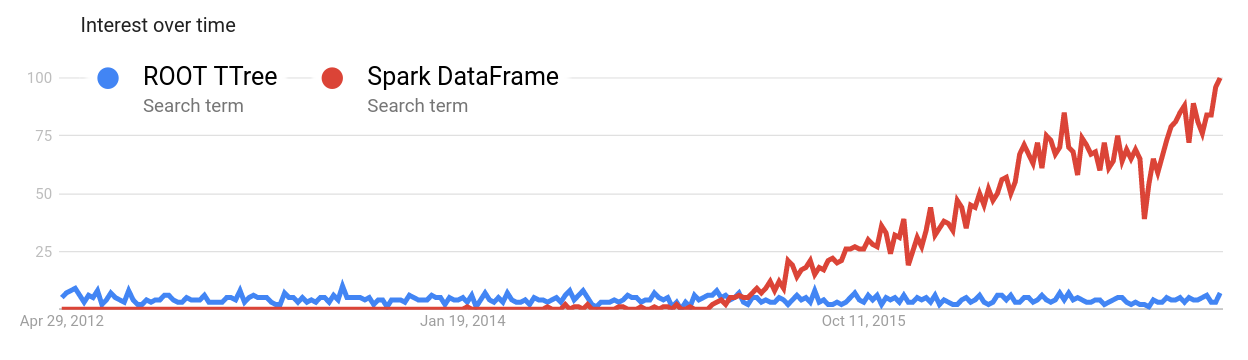
\includegraphics[width=\linewidth]{root-spark-google-trends.png}

%% \vfill
%% \textcolor{darkblue}{Question-and-answer sites:}
%% \begin{itemize}
%% \item RootTalk: 14,399 threads in 1997--2012 (15 years)
%% \item StackOverflow questions tagged \#spark: 26,155 in the 3.3 years it has existed.
%% \end{itemize}

%% \vfill
%% \textcolor{darkblue}{More users to talk to; more developers adding features/fixing bugs.}
%% \end{frame}

%% \begin{frame}{Building bridges: low effort-to-reward}
%% \vspace{0.5 cm}
%% \begin{center}
%% \hspace{1 cm}\only<1>{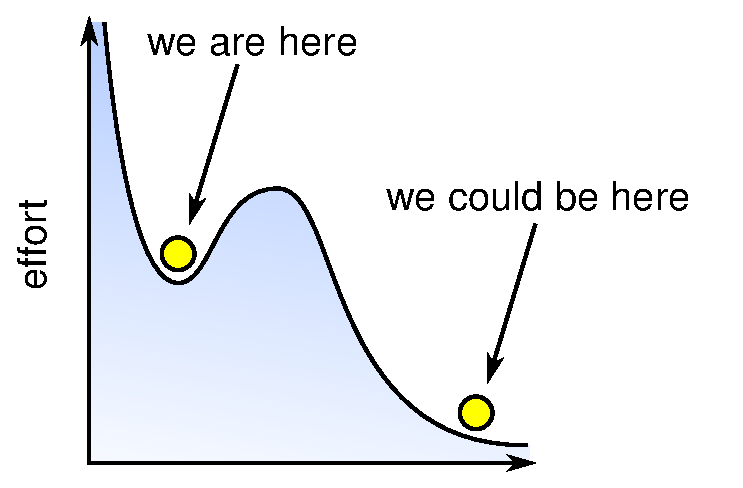
\includegraphics[width=0.75\linewidth]{effort0.pdf}}\only<2>{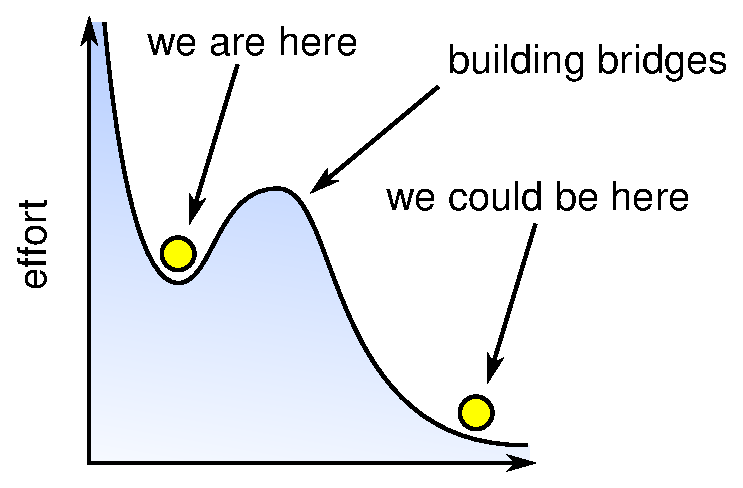
\includegraphics[width=0.75\linewidth]{effort.pdf}}
%% \end{center}
%% \end{frame}

%% \begin{frame}{Who am I?}
%% \begin{columns}[t]
%% \column{0.55\linewidth}
%% \begin{columns}
%% \column{0.4\linewidth}
%% Jim Pivarski
%% \column{0.2\linewidth}
%% \hspace{-1.3 cm}
\includegraphics[width=\linewidth]{faces/jim_pivarski.png}
%% \end{columns}

%% \begin{itemize}
%% \item 5 years CLEO (9 GeV $e^+e^-$)
%% \item 5 years CMS (7 TeV $pp$)
%% \item \only<1>{5 years Open Data Group}\only<2>{\mbox{\textcolor{darkblue}{5 years Open Data Group \hspace{0.4 cm}$\longrightarrow$\hspace{-3 cm}}}}
%% \item 1+ years Project DIANA-HEP
%% \end{itemize}

%% \column{0.5\linewidth}
%% \uncover<2>{\textcolor{darkblue}{
%% hyperspectral imagery \\
%% automobile traffic \\
%% network security \\
%% Twitter sentiment \\
%% Google n-grams \\
%% DNA sequence analysis \\
%% credit card fraud detection
%% }}

%% \uncover<2>{\Large\textcolor{darkblue}{ and ``Big Data'' tools}}
%% \end{columns}
%% \end{frame}

%% \begin{frame}{}

%% \only<1>{\mbox{\hspace{-1 cm}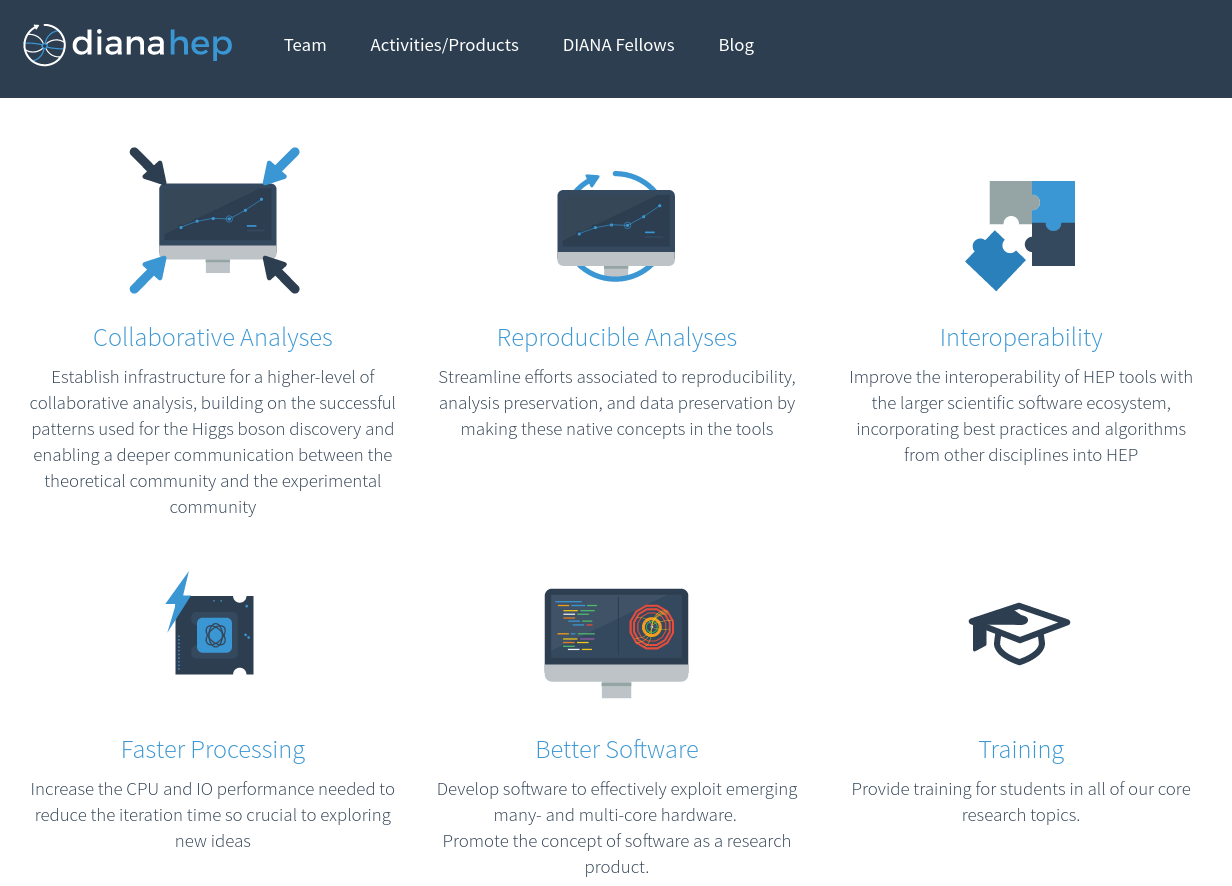
\includegraphics[width=1.2\linewidth]{diana-hep.png}}}
%% \only<2>{\mbox{\hspace{-1 cm}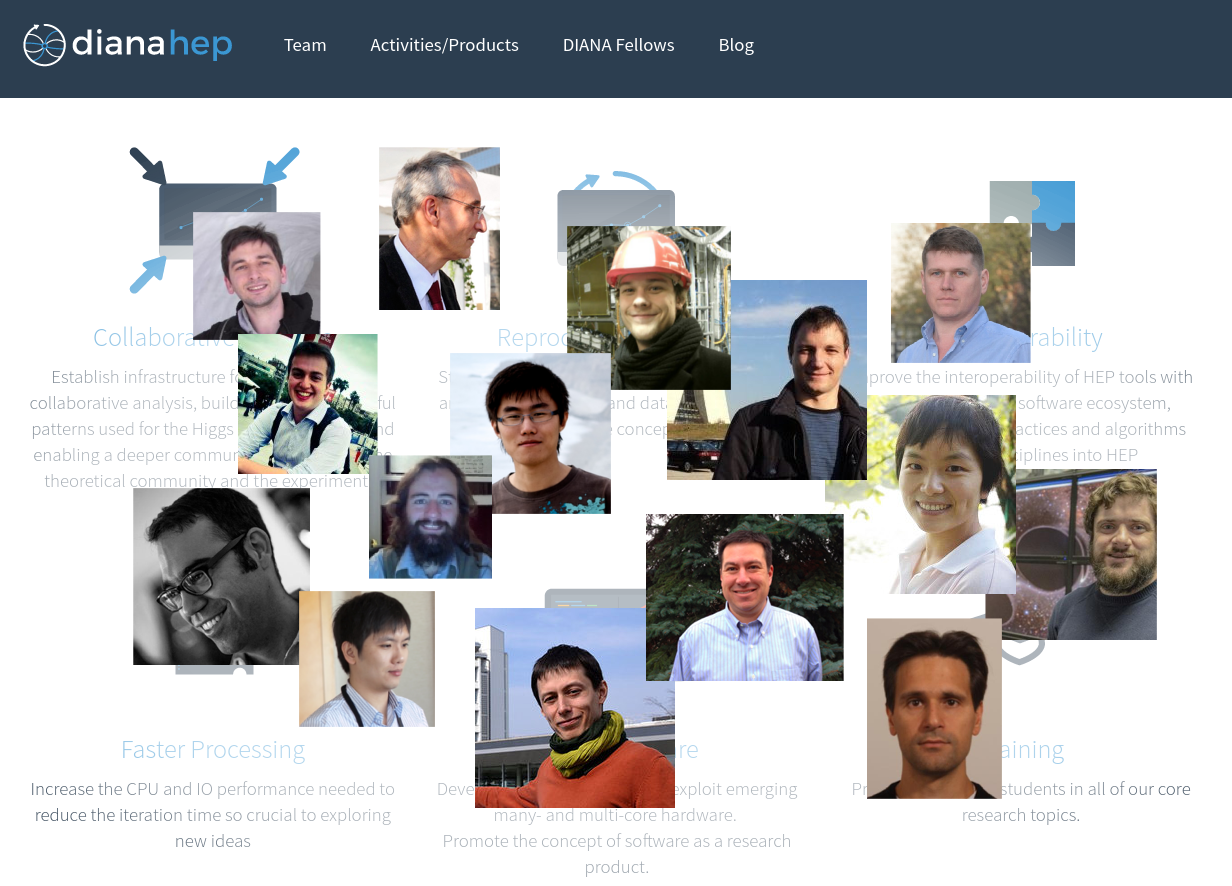
\includegraphics[width=1.2\linewidth]{diana-hep2.png}}}

%% \end{frame}

%% \begin{frame}{Outline of this talk}
%% \Large
%% \begin{description}\setlength{\itemsep}{0.5 cm}
%% \item[Data plumbing:] a CMS analysis in Apache Spark
%% \item[Histogrammar:] HEP-like tools in a functional world
%% \item[Femtocode:] the ``query system'' concept in HEP
%% \end{description}
%% \end{frame}

%% \begin{frame}{Apache Spark}
%% \vspace{0.5 cm}
%% 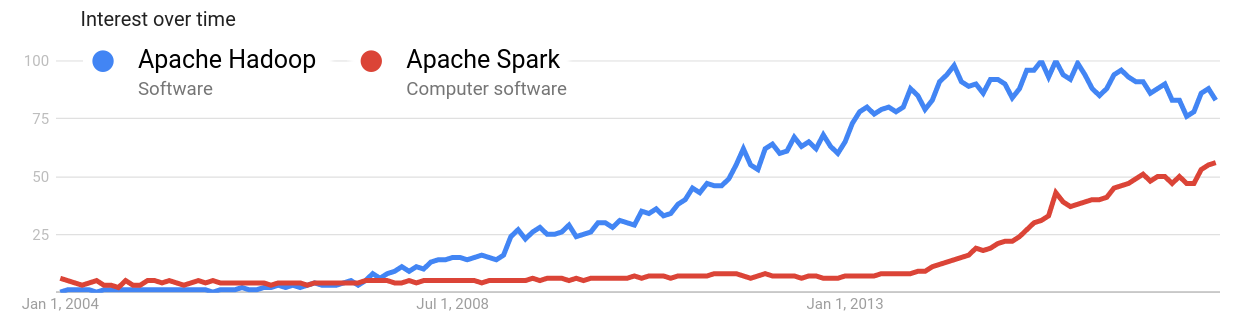
\includegraphics[width=\linewidth]{hadoop-versus-spark.png}

%% \vfill
%% 
\includegraphics[width=0.25\linewidth]{spark.png}

%% \begin{itemize}
%% \item Like Hadoop in that it implements map-reduce, but these are just two out of many functionals.
%% \item<2-> Not a competitor to Hadoop: can run on a Hadoop cluster.
%% \item<3-> Primary interface is a commandline console. Each command does a distributed job and returns a result, while-you-wait\texttrademark.
%% \item<4-> User controls in-memory cache on the cluster, effectively getting an $\mathcal{O}(\mbox{TB})$ working space in RAM.
%% \end{itemize}
%% \end{frame}

%% \begin{frame}{CMS analysis on Spark}
%% \vfill
%% \begin{itemize}
%% \item Oliver Gutsche, Matteo Cremonesi, Cristina Su\'arez (Fermilab) wanted to try their CMS dark matter search on Spark.
%% \item This was my first project with DIANA-HEP: I joined to plow through technical issues before the analysts hit them.

%% \vfill
%% \begin{center}
%% 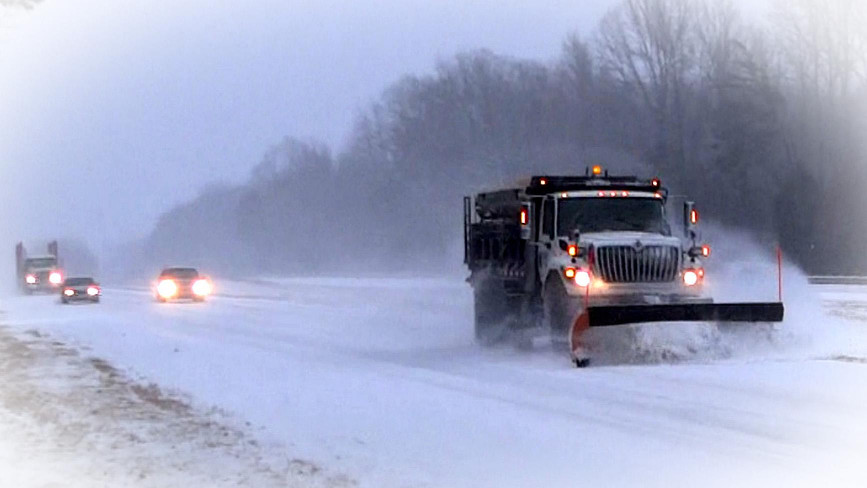
\includegraphics[width=0.75\linewidth]{snowplow.jpg}
%% \end{center}
%% \end{itemize}
%% \end{frame}

%% \begin{frame}{Problems!}
%% \Large

%% \begin{enumerate}\setlength{\itemsep}{0.5 cm}
%% \item Need a Spark cluster.

%% \item Spark, like most ``Big Data'' tools, runs on the Java Virtual Machine (JVM), not C++, and doesn't recognize our ROOT data format.

%% \item HEP analysis tools like histograms don't have the right API to fit Spark's functional interface.

%% \end{enumerate}
%% \end{frame}

%% \begin{frame}{\#1. Need a Spark cluster}
%% Several other groups are interested in this and were willing to share resources in exchange for having us test their system.

%% \begin{itemize}
%% \item Alexey Svyatkovskiy (Princeton) was active in the group, helping us use the Princeton BigData cluster.
%% \item Saba Sehrish and Jim Kowalkowski (Fermilab) modified the analysis for NERSC.
%% \item Maria Girone, Luca Canali, Kacper Surdy (CERN), and Vaggelis Motesnitsalis (Intel) are now setting up a Data Reduction Facility at CERN as an OpenLab project.
%% \item Offer from Marco Zanetti and Mauro Morandin at Padua.
%% \end{itemize}
%% \end{frame}

%% \begin{frame}{\#2. Getting data from ROOT files into JVM}
%% \vspace{0.5 cm}
%% \small

%% \textcolor{darkblue}{\normalsize A run-down of the attempted solutions\ldots}
%% \begin{enumerate}
%% \item \textcolor{darkblue}{Java Native Interface (JNI)} \\ No! This ought to be the right solution, but Java \\ and ROOT are both large, complex applications \\ with their own memory management: couldn't keep \\ them from interfering (segmentation faults).

%% \vspace{-2.2 cm}
%% \hfill 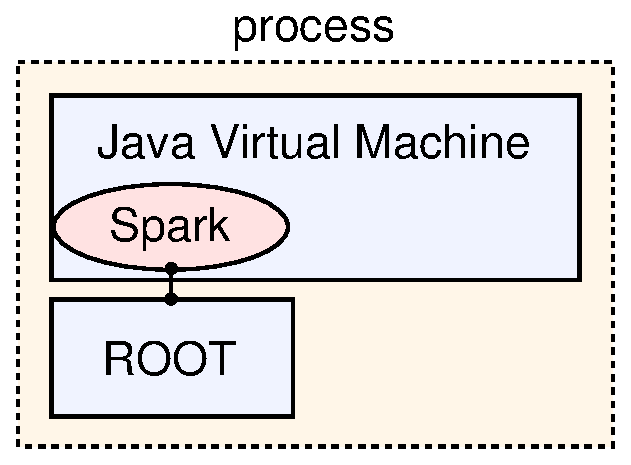
\includegraphics[height=1.65 cm]{root-spark.pdf}

%% \vspace{0.5 cm}
%% \item \textcolor{darkblue}{\normalsize Python as glue: PyROOT and PySpark in the same process}

%% \hfill 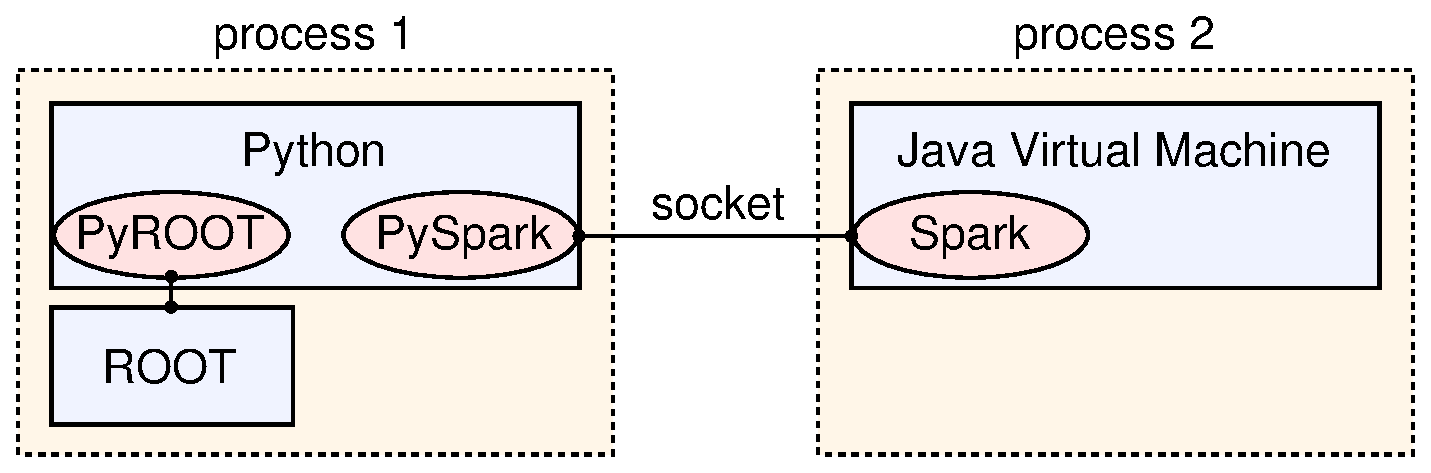
\includegraphics[height=1.65 cm]{pyroot-pyspark.pdf}

%% \vspace{-1.8 cm}
%% PySpark is a low-performance \\ solution: all data must be passed \\ over a text-based socket and \\ interpreted by Python.

%% \item \textcolor{darkblue}{\normalsize Convert to a Spark-friendly format, like Apache Avro}

%% We used this for a year. Efficient after conversion, but conversion step is awkward. Avro's C library is difficult to deploy.

%% \item \textcolor{darkblue}{\normalsize Use pure Java code to read ROOT files}

%% What we do now. It's worth it.

%% \end{enumerate}
%% \end{frame}

%% \begin{frame}{}

%% \only<1>{{\mbox{\hspace{-1 cm}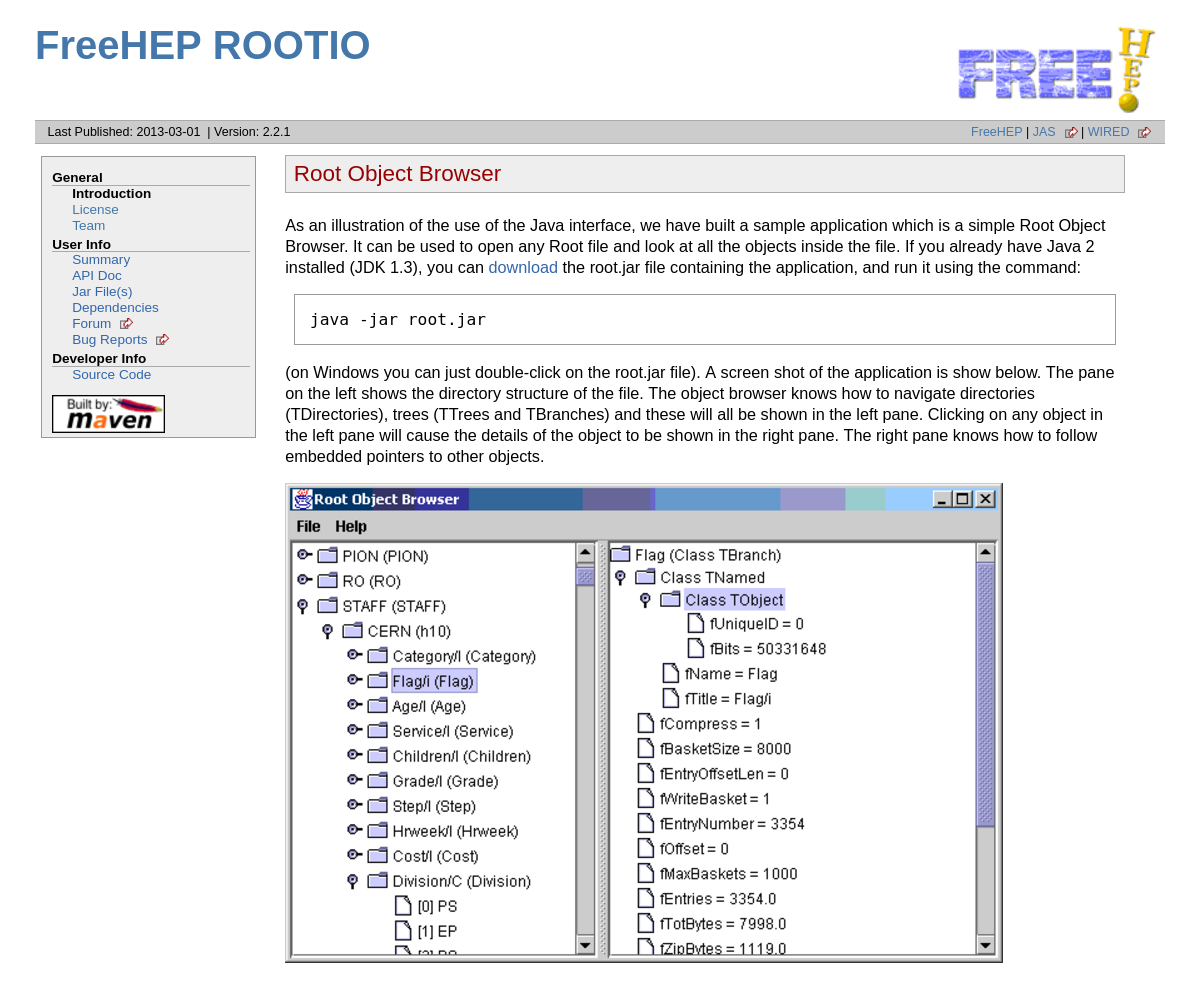
\includegraphics[width=1.2\linewidth]{rootio-screenshot.png}}}}
%% \only<2->{{\mbox{\hspace{-1 cm}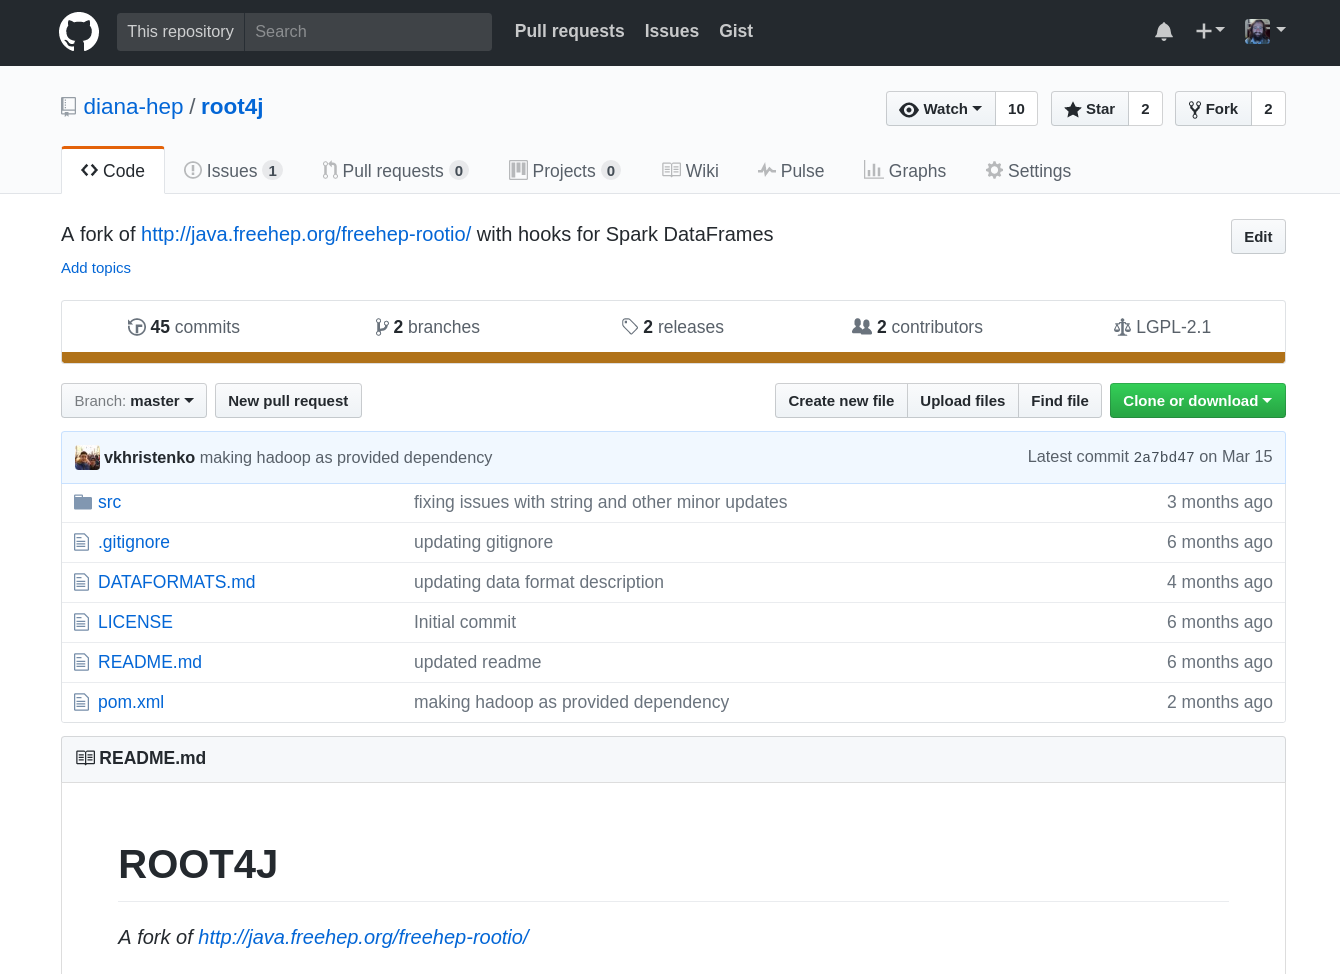
\includegraphics[width=1.2\linewidth]{root4j.png}}}}

%% \begin{onlyenv}<3>
%% \vspace{-3.5 cm}\hfill\begin{minipage}{3 cm}
%% \begin{center}
%% 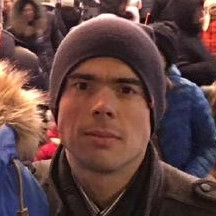
\includegraphics[width=2 cm]{viktor.jpg}

%% Viktor Khristenko

%% {\small University of Iowa}
%% \end{center}
%% \end{minipage}\hspace{1 cm}\vspace{3.5 cm}
%% \end{onlyenv}

%% \end{frame}

%% \begin{frame}[fragile]{Problem \#3. Histogram interface}
%% \vspace{0.4 cm}
%% \textcolor{darkblue}{This is how Spark processes data:}

%% \small
%% \begin{minted}{scala}
%% val final_counter =
%%     dataset.filter(event => event.goodness > 2)
%%            .map(event => do_something(event.muons))
%%            .aggregate(empty_counter)(
%%       (counter, result) => increment(counter, result),
%%       (c1, c2) => combine(c1, c2))
%% \end{minted}

%% \begin{uncoverenv}<2->
%% Read as a chain from top to bottom:
%% \begin{enumerate}\setlength{\itemsep}{-0.1 cm}
%% \item Start with {\tt\small dataset} on the cluster somewhere.
%% \item Filter it with {\tt\small event.goodness > 2}.
%% \item Compute {\tt\small do\_something} on each event's muons.
%% \item Accumulate some counter (e.g.\ histogram or other data summary), starting with {\tt\small empty\_counter}, using {\tt\small increment} to fill with each event's {\tt\small result}, combining partial results with {\tt\small combine}.
%% \end{enumerate}
%% all distributed across the cluster, returning only {\tt\small final\_counter}.
%% \end{uncoverenv}
%% \end{frame}

%% \begin{frame}[fragile]{Problem \#3. Histogram interface}
%% \vspace{0.4 cm}
%% \textcolor{darkblue}{This is how ROOT/PAW/HBOOK histograms expect to be called:}

%% \small
%% \begin{minted}{c++}
%% // on a worker handling one partition of data
%% hist = new TH1F("name", "title", numBins, low, high);

%% for (i = start_partition;  i < end_partition;  i++) {
%%     dataset.GetEntry(i);
%%     if (goodness > 2)
%%         hist->Fill(do_something(muons));
%% }

%% // on the head node, after downloading partial hists
%% hadd(hists);
%% \end{minted}
%% \end{frame}

%% \begin{frame}[fragile]{Problem \#3. Histogram interface}
%% \vspace{0.4 cm}
%% \textcolor{darkblue}{Trying to wedge the square peg into the round hole:}

%% \small
%% \begin{minted}{python}
%% import ROOT
%% empty_hist = ROOT.TH1F("n", "t", numBins, low, high)

%% def increment(hist, result):
%%     hist.Fill(result)
%%     return hist

%% def combine(h1, h2):
%%     return h1.Add(h2)

%% filled_hist =
%%   data.filter(lambda event: event.goodness > 2)     \
%%       .map(lambda event: do_something(event.muons)) \
%%       .aggregate(empty_hist, increment, combine)
%% \end{minted}
%% \end{frame}

%% \begin{frame}{}
%% \begin{center}
%% \vfill
%% \large \textcolor{darkblue}{It's not impossible, but it's awkward.}

%% \vfill
%% \textcolor{darkblue}{Awkward is bad for data analysis because you really should be focusing on the complexities of your analysis, not your tools.}

%% \vfill
%% \end{center}
%% \end{frame}

%% \begin{frame}[fragile]{Making histograms functional}
%% There's a natural way to do histograms in functional programming: add a fill rule to the declaration.

%% \small
%% \begin{minted}{python}
%% hist = Histogram(numBins, low, high,
%%                      lambda event: event.what_to_fill)
%% \end{minted}
%% \normalsize

%% \vfill
%% \begin{uncoverenv}<2->
%% This way, {\tt\small what\_to\_fill} doesn't have to be specified in the (non-existent) ``for'' loop.

%% \small
%% \begin{minted}{python}
%% dataset.fill_it_for_me(hist)
%% \end{minted}
%% \end{uncoverenv}
%% \end{frame}

%% \begin{frame}[fragile]{It's cooler this way}
%% \vfill
%% \textcolor{darkblue}{Functional programming emphasizes composition: building new functionality by composing functions.}

%% \vfill
%% \small
%% \begin{onlyenv}<1>
%% \begin{minted}{python}
%% # standard 1-D histogram
%% Bin(numBins, low, high, x_rule, Count())
%% \end{minted}
%% \begin{itemize}
%% \item {\tt\small Bin} splits into bins by {\tt\small x\_rule}, passes to a {\tt\small Count} in each bin,
%% \item {\tt\small Count} counts.
%% \end{itemize}
%% \end{onlyenv}
%% \begin{onlyenv}<2>
%% \begin{minted}{python}
%% # profile plot
%% Bin(numBins, low, high, x_rule, Deviate(y_rule))
%% \end{minted}
%% \begin{itemize}
%% \item {\tt\small Bin} splits into bins by {\tt\small x\_rule}, passes to a {\tt\small Deviate} in each bin,
%% \item {\tt\small Deviate} computes the mean and standard deviation of {\tt\small y\_rule}.
%% \end{itemize}
%% \end{onlyenv}
%% \begin{onlyenv}<3>
%% \begin{minted}{python}
%% # 2-D histogram
%% Bin(numBins, low, high, x_rule,
%%     Bin(numBins, low, high, y_rule,
%%         Count()))
%% \end{minted}
%% \begin{itemize}
%% \item {\tt\small Bin} splits into bins by {\tt\small x\_rule}, passes to a {\tt\small Bin} in each bin,
%% \item second {\tt\small Bin} does the same with {\tt\small y\_rule}.
%% \end{itemize}
%% \end{onlyenv}
%% \begin{onlyenv}<4>
%% \begin{minted}{python}
%% # different binning methods on different dimensions
%% Categorize(event_type,
%%     SparselyBin(trigger_bits,
%%         IrregularlyBin([-2.4, -1.5, 1.5, 2.4], eta,
%%             Bin(100, 0, 100, pt,
%%                 Count()))))
%% \end{minted}
%% \begin{itemize}
%% \item {\tt\small Categorize} splits based on string value (like a bar chart)
%% \item {\tt\small SparselyBin} only creates bins if their content is non-zero
%% \item {\tt\small IrregularlyBin} lets you place bin edges anywhere
%% \end{itemize}\end{onlyenv}
%% \begin{onlyenv}<5>
%% \begin{minted}{python}
%% # bundle histograms to be filled together
%% Bundle(
%%     one = Bin(numBins, low, high, fill_one),
%%     two = Bin(numBins, low, high, fill_two),
%%     three = Bin(numBins, low, high, fill_three))
%% \end{minted}
%% \begin{itemize}
%% \item {\tt\small Bundle} is a directory mapping names to aggregators; same interface as all the other aggregators
%% \end{itemize}\end{onlyenv}
%% \begin{onlyenv}<6>
%% \begin{minted}{python}
%% # to organize your analysis

%% pack_o_plots = Bundle(
%%     one = Bin(numBins, low, high, fill_one),
%%     two = Bin(numBins, low, high, fill_two))

%% Bundle(
%%     withcut = Select(cut_rule, pack_o_plots),
%%     nocut   =                  pack_o_plots)
%% \end{minted}
%% \begin{itemize}
%% \item {\tt\small Select} only passes down events that pass {\tt\small cut\_rule}
%% \item {\tt\small Bundles} are now nested like subdirectories, one {\tt\small pack\_o\_plots} with cut, the other without
%% \end{itemize}\end{onlyenv}
%% \begin{onlyenv}<7>
%% \begin{minted}{python}
%% # or do wacky things
%% Bin(numBins, low, high, lambda event: event.x,
%%     Bundle(
%%         nonzero = Fraction(lambda event: event.y > 0,
%%                            Count()),
%%         mean = Average(lambda event: event.y),
%%         max = Maximize(lambda event: event.y)))
%% \end{minted}
%% \begin{itemize}
%% \item fills a {\it directory} of ``nonzero,'' ``mean,'' and ``max'' in each {\it bin} of x.
%% \end{itemize}\end{onlyenv}
%% \end{frame}

%% \begin{frame}{}

%% {\mbox{\hspace{-1 cm}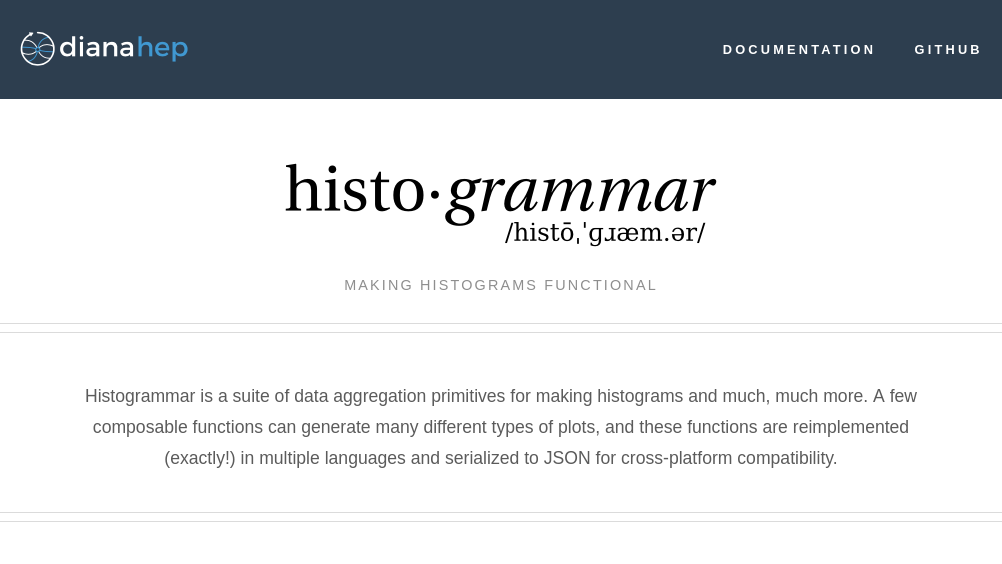
\includegraphics[width=1.2\linewidth]{frontpage.png}}}

%% \vspace{0.5 cm}
%% See \textcolor{blue}{\underline{\url{http://histogrammar.org}}} for more.

%% \vspace{1.5 cm}
%% \end{frame}

\begin{frame}{}

{\mbox{\hspace{-1 cm}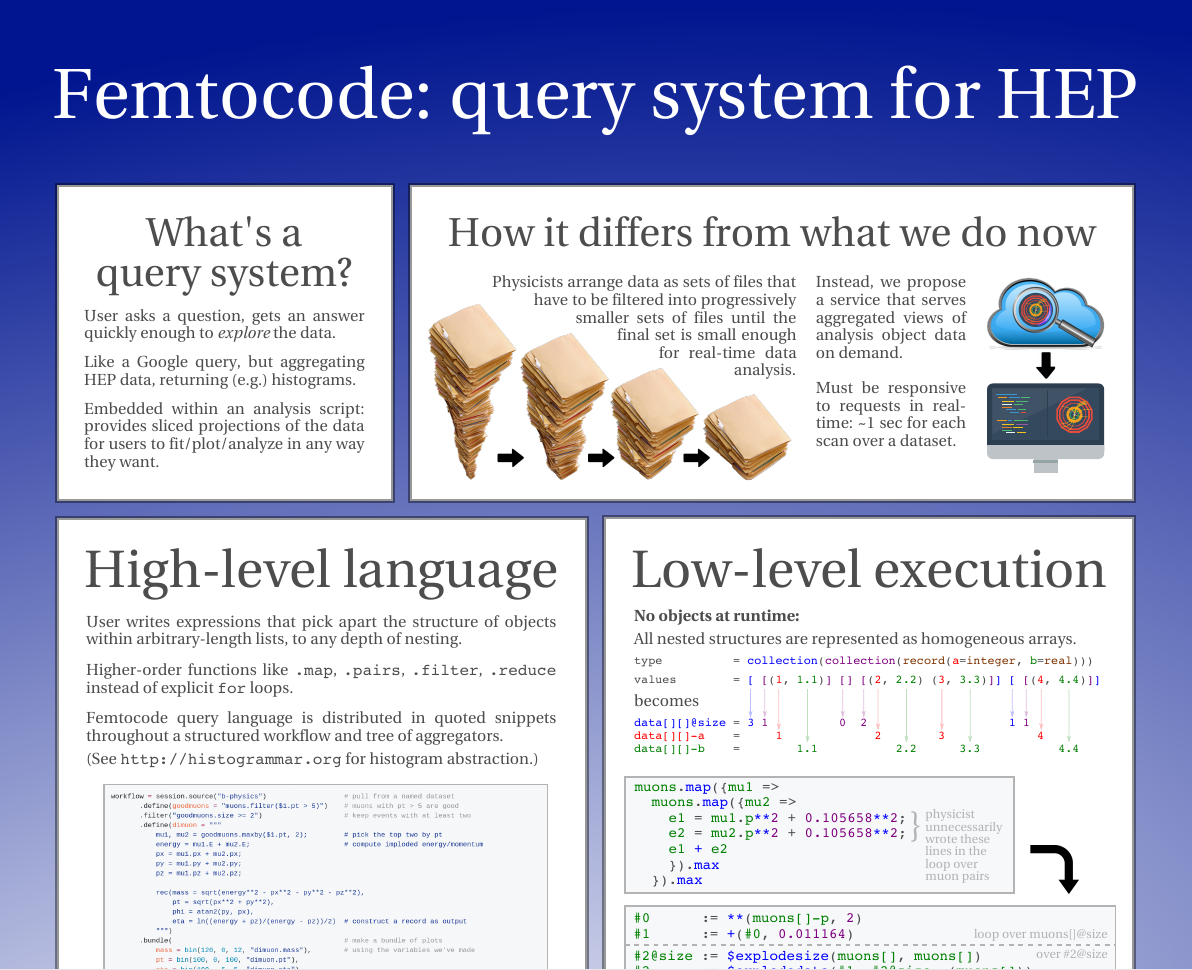
\includegraphics[width=1.2\linewidth]{femtocode.png}}}

\end{frame}

\end{document}
